\documentclass{beamer}

\usepackage{graphicx}
\usepackage{booktabs}

\title[SDES Project 2]{Handwritten digit recognition using Neural Networks}
\author{Harish Murali \& Surya Mohan}
\institute[iitb]
{
IIT Bombay
}
\date{\today}

\begin{document}

%------------------------------------------------

\begin{frame}
\titlepage
\end{frame}

%------------------------------------------------

\begin{frame}
\frametitle{Introduction}
Neural Networks are bio mimicking algorithms which attempt to imitate the functionality of a human mind. A neural network consists of multiple layers of neurons which take some input and perform linear transformations on these to produce the required output.
\\~\\
Each layer of neurons receives computes its output by taking linear combinations of the output of the layer preceding it. The primary goal in implementing a Neural network therefore is to compute the weights and biases which are the parameters of the transformation.
\end{frame}

%------------------------------------------------

\begin{frame}
\frametitle{Layout of a generic Neural network}
\begin{figure}
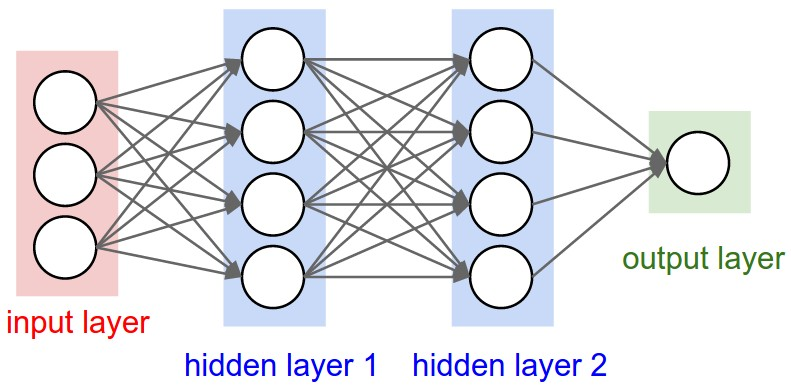
\includegraphics[width=0.8\linewidth]{nn}
\\
\caption{Source: http://cs231n.github.io/neural-networks-1/}
\end{figure}
\end{frame}

%------------------------------------------------

\begin{frame}
\frametitle{Continued}
\begin{itemize}
\item Each neuron in the subsequent layers is computed as a linear combination of the neurons of the previous layer.
\item The coefficients of this linear combination are called the weights
\item We also add biases to the network to ensure that the output of a zero input is not constrained to be zero.
\item The outputs of each layer are called activations. The weighted input to a layer, denoted by $z^l$ is simply the linear combination described above. We apply a non linear activation function to this to obtain an output acivation, denoted by $a^l$ in the range of 0 to 1, which can conveniently be interpreted as a probability
\\~\\
\begin{center}
$a_i^l = \sigma(\Sigma_j w_{ij}^{l-1}a_j^{l-1} + b_i^l)$\\
where $\sigma(z) = \frac{1}{1+e^{-z}}$
\end{center}
\end{itemize}
\end{frame}

%------------------------------------------------

\begin{frame}
\frametitle{Training a Neural Network}
\begin{itemize}
\item We define a cost function which is a measure of how far away the computed solution is from the expected solution. For this assignment, we have used a quadratic cost function.
\item The objective therefore is to use an optimisation algorithm to minimise this cost function.
\begin{center}
$J = \frac{1}{2} \Sigma_j ||y_j - a_j||^2$ 
\end{center}
where $y$ is the expected output \\~\\

\item Computing the gradient of the cost function, i.e. the set of partial derivatives of the cost function with respect to the weights and biases of the network is the critical part.
\item Once we have the derivatives, a straight forward implementations of gradient descent will do the job.
\end{itemize}
\end{frame}

%------------------------------------------------

\begin{frame}
\frametitle{Backpropagation Algorithm}
\begin{itemize}
\item The backpropagation algorithm enables us to compute the gradient of the cost function.
\item The important idea is that once we compute the expected output, the error in the final layer and thus the partial derivatives of the cost w.r.t the output layer weights can be computed.
\item We now backpropagate these errors to compute all the other derivatives using the chain rule.\\
\begin{center}
$\delta^L = \nabla J \cdot \sigma'(z^L)$\\
$\delta^l = ((w^{l+1})^T \delta^{l+1}) \cdot \sigma'(z^l)$\\
$\frac{\partial J}{\partial w^l_{jk}} = a^{l-1}_k \delta^l_j$\\
$\frac{\partial J}{\partial b} = \delta$
\end{center}

\end{itemize}
\end{frame}

%------------------------------------------------

\begin{frame}
\frametitle{Visualising the image data}
We have used the MNIST handwritten image dataset to train our neural network. The dataset has 60,000 images for training
\begin{figure}
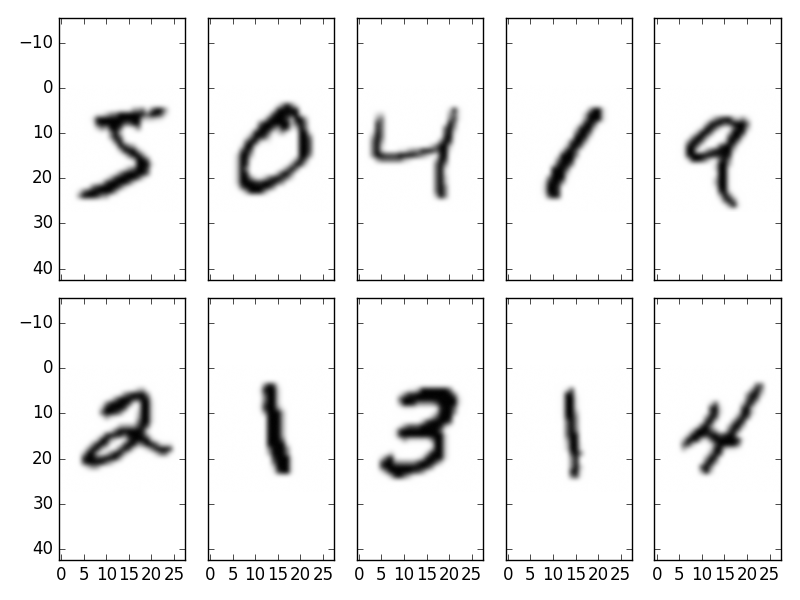
\includegraphics[width=0.8\linewidth]{numbers}
\caption{Source of the data file: http://yann.lecun.com/exdb/mnist/}
\end{figure}
\end{frame}

%------------------------------------------------

\begin{frame}
\begin{itemize}
\item We trained the neural network in about 50 iterations and it predicted the correct result 91\% the time.
\item There are several parameters that can be tuned for instance, the number of layers in the network, the learning rate in the gradient descent algorithm, number of training examples per batch in the Stochastic Gradient Descent Algorithm we used.
\item The accuracy of the neural network predictions also depends heavily on the preprocessing of the image data. When the input is unprocessed images, with pixel values in the range 0-256, the learning is very poor. This is because the sigmoid function is extremely sensitive and saturates for inputs greater than 37 and also the gradients which are functions the sigmoid derivative are very close to zero.
\item So, what need to be done is the image data must be shifted so that the mean is at 0 and the range is between 0 and 1. This alone leads to an improvement of accuracy from 20-30\% to 90\%
\end{itemize}
\end{frame}
\end{document}